\section{Accelerating Applications}
The application of accelerated approaches in the scientific discovery cycle (see \Cref{fig:applications}) hinges on their ability to streamline and enhance each stage of the process.
However, a fundamental challenge in effectively implementing these approaches lies in the choice of machine-readable representation.

This challenge is particularly evident in the representation of molecules and materials, which must balance computational efficiency with the preservation of structural, compositional, and functional properties. 
Take, for example, the high-temperature superconductor \ce{YBa2Cu3O_{7-x}}. 
While atomic positions and coordinates are theoretically sufficient to solve the Schrödinger equation and describe this material, such a representation may not provide the adaptability necessary for diverse tasks. What defines a good representation depends on the problem. \autocite{huang2016understanding}. 
A representation designed to predict critical temperature must efficiently encode the relationship between oxygen stoichiometry and superconducting properties, emphasizing features like oxygen vacancy patterns and charge transfer mechanisms. 
Conversely, a representation for structural stability might prioritize different geometric or bonding characteristics.

This tension has led to three primary strategies for representing molecules and materials (read \Cref{sec:common_representations} to learn in detail about the different representations that currently exist). 
First, domain-specific text-based formats---such as \gls{smiles} \autocite{weininger1988smiles}, \gls{selfies} \autocite{krenn2020self}, and \gls{cif} \autocite{hall1991crystallographic}---offer compact, machine-readable encodings of structural information. While these necessarily omit certain physical details, their computational tractability has enabled breakthroughs, as demonstrated by \textcite{jablonka2024leveraging} in their \gls{llm}-based generation of valid molecular and material structures.

Yet, the question remains: Which representation is optimal for a given task? Future advances in accelerated discovery will likely hinge on adaptive representations that dynamically balance these competing demands.

\subsection{Property Prediction} \label{sec:prediction}

\glspl{gpm} have emerged as a powerful tool for predicting molecular and material properties, offering an alternative to traditional quantum mechanical calculations or specialized \gls{ml} models. 
Current \gls{gpm}-driven property prediction tasks span both classification and regression. 
Unlike conventional approaches that rely on task-specific architectures and extensively labeled data, \glspl{gpm} have demonstrated strong generalization capabilities across diverse domains, efficiently adapting to various prediction tasks. 
Their success extends to multiple datasets, from standardized benchmarks such as \modelname{MoleculeNet} \autocite{wu2018moleculenet}, to curated datasets targeting specific applications such as antibacterial activity \autocite{chithrananda2020chemberta} or photovoltaic efficiency\autocite{aneesh2025semantic}.

Three key methodologies have been explored to adapt \glspl{llm} for property prediction: prompting techniques (see \Cref{sec:prompting}), fine-tuning (see \Cref{sec:fine-tuning}) on domain-specific data, and \gls{rag} (see \Cref{sec:rag}) approaches that combine \glspl{llm} with external knowledge bases. 

\begin{table}[htbp]
    \centering
    \caption{\textbf{Non-comprehensive list of \glspl{gpm} applied to property prediction tasks}. The table presents different models and their applications across different molecular and materials property prediction benchmarks, showing the diversity of properties (from molecular toxicology to crystal band gaps), datasets used for evaluation, modeling approaches (prompting, fine-tuning, or retrieval-augmented generation), and task types (classification or regression.)}
    \label{tab:property_prediction_models}
    \resizebox{\textwidth}{!}{%
    \begin{tabular}{lllcc}
        \toprule
        \textbf{Model} & \textbf{Property} & \textbf{Dataset} & \textbf{Approach}  & \textbf{Task}\\
        \midrule
        \multirow{7}{*}{GPT-Chem\autocite{jablonka2024leveraging}} & HOMO/LUMO & QMUGs\autocite{isert_qmugs_2022} & \multirow{7}{*}{FT} & C, R \\
        & Solubility & DLS-100\autocite{mitchell_dls-100_2017} & & C, R \\
        & Lipophilicity & LipoData\autocite{jablonka2024leveraging} & & C, R \\
        & Hydration Free Energy & FreeSolv\autocite{mobley_freesolv_2014} & & C, R \\
        & Photoconversion Efficiency & OPV\autocite{jablonka2024leveraging} & & C, R  \\
        & Toxicology & Tox21\autocite{richard_tox21_2021} & & C, R  \\
        & $\text{CO}_2$ Henry Coefficients of MOFs & MOFSorb-H\autocite{lin_silico_2012} & & C, R \\
        \cmidrule{1-5}
        \multirow{3}{*}{LLM-Prop\autocite{rubungo_llm-prop_2023}} & Band Gap & \multirow{3}{*}{CrystalFeatures-MP2022\autocite{rubungo_llm-prop_2023}} & \multirow{3}{*}{P} &  R  \\
        & Volume & & & R \\
        & Is the band gap direct?&  & & C \\
        \midrule
        \multirow{12}{*}{LLM4SD\autocite{zheng2025large}} & Blood-brain barrier penetration & BBBP\autocite{sakiyama_prediction_2021} & \multirow{10}{*}{P} & C \\
        & FDA approval & ClinTox\autocite{wu2018moleculenet} & & C \\
        & Toxicology & Tox21\autocite{richard_tox21_2021} & & C \\
        & Drug-related side effects & SIDER\autocite{kuhn_sider_2016} & & C \\
        & HIV replication inhibition & HIV\autocite{wu2018moleculenet} & & C \\
        & $\beta$-secretase binding & BACE\autocite{wu2018moleculenet} & & C \\
        & Solubility & ESOL\autocite{wu2018moleculenet} & & R \\
        & Hydration Free Energy & FreeSolv\autocite{mobley_freesolv_2014} & & R \\
        & Lipophilicity & Lipophilicity\autocite{wu2018moleculenet} & & R \\
        & Quantum Mechanics & QM9\autocite{wu2018moleculenet} & & R \\
        \midrule
        \multirow{4}{*}{\modelname{LLaMP\autocite{chiang2024llamp}}} & Bulk modulus & \multirow{4}{*}{Materials Project\autocite{riebesell2025framework}} & \multirow{4}{*}{RAG} & R \\
        & Formation energy & & & R \\
        & Electronic bandgap & & & R \\
        & Multi-element electronic bandgap & & & R \\
        \bottomrule
    \end{tabular}
    }
    \vspace{0.5em}
    \footnotesize
    \begin{minipage}{\linewidth}
        \textbf{Key:}  P = prompting; FT = fine-tuned model; RAG = retrieval-augmented generation; C = Classification; R = Regression
    \end{minipage}
\end{table}

\subsubsection{Prompting} 
Prompt engineering involves designing targeted instructions to guide \glspl{gpm} in performing specialized tasks without altering their underlying parameters by leveraging their embedded knowledge. 
In molecular and materials science, this strategy goes beyond simply asking a model to predict properties. 
It also includes carefully structured prompts to elicit detailed molecular and material descriptions directly from the model's pre-trained knowledge.

\textcite{liu2025integrating} conducted a comprehensive evaluation of different prompting techniques to predict the properties of organic small molecules and crystal materials. 
Some of these techniques included domain-knowledge (prior knowledge was embedded in the prompt), expert (role-play instructions), and few-shot \gls{cot} (the text\textit{\enquote{Let's think step by step}} is added) prompting. 
Of these, domain knowledge achieved maximum performance. However, their evaluation was limited to a relatively small set of molecules and tasks, and the effectiveness of their domain-knowledge approach may not generalize to other molecular property domains.

Building on these foundational prompting strategies, few-shot prompting approaches leverage \gls{icl} to enhance performance through selected examples \textcite{liu2024moleculargpt} used \gls{smiles} string representations of molecules with few-shot \gls{icl}, retrieving structurally similar molecules as demonstrations to enhance property prediction. 
This approach highlights how \gls{icl} can transfer knowledge from similar molecule examples without requiring model fine-tuning for each task. 
However, the effectiveness of \gls{icl} depends on the quality of retrieved examples.

\textcite{fifty2023incontext} moved beyond direct text prompting of molecules and introduced \gls{camp}: an \gls{icl} algorithm that uses a two-stage encoding approach without relying on pre-trained \glspl{llm}.
First, a specialized \gls{mpnn} encodes molecule graphs into molecular embeddings rather than processing them as raw text. 
These embeddings are then fed into a transformer encoder, which learns contextualized representations across the support set (a small collection of labeled molecule-property pairs) and the unlabeled query molecules. They demonstrated \gls{camp}'s ability to outperform existing few-shot learning baselines by providing relevant molecular examples within the prompt context. However, this approach is constrained by the context-length limitations of the underlying \glspl{lm} and the challenge of selecting optimal demonstration examples.

More sophisticated approaches have leveraged prompting as part of multi-modal frameworks. The \modelname{LLM4SD} pipeline by \textcite{zheng2025large} employs specialized prompts to guide \glspl{lm} through their pre-trained knowledge on scientific literature, generating known rules (e.g., molecules weighing under \SI{500}{Da} are more likely to pass the blood-brain barrier) that transform molecules into feature vectors (e.g. \ce{CCO} could translate to a vector $[2,46.07,1,1]$ where each number represents a feature of the molecule, in this example [\# \ce{C}, MW, \# \ce{H}-bond donors, \# \ce{H}-bond acceptors]) for use with a random forest model, which they consider \enquote{interpretable}. 
This approach outperformed specialized \gls{sota} models across $58$ benchmark tasks, while providing interpretable reasoning about prediction logic (see \Cref{tab:property_prediction_models} for properties predicted by this model). However, its reliance on rule extraction may limit its ability to capture complex, non-linear relationships that specialized deep learning models can identify.

\paragraph{\glspl{llm} as Feature Extractors} Another emerging application of \glspl{llm} is their use as \enquote{feature extractors}, where they generate textual or embedded representations of molecules or materials. For instance, in materials science, \textcite{aneesh2025semantic} employed \glspl{llm} to generate text embeddings of perovskite solar cell compositions. 
These embeddings were subsequently used to train a \gls{gnn} for predicting power conversion efficiency, demonstrating the potential of \glspl{llm} to enhance feature representation in materials informatics. 
Similarly, in the molecular domain, \textcite{srinivas2024crossmodal} used zero-shot \gls{llm} prompting (see \Cref{box: cot_prompting} for prompt examples) to generate detailed textual descriptions of molecular functional groups, which are used to train a small \gls{lm}. This \gls{lm} is used to compute text-level embeddings of molecules. Simultaneously, they generate molecular graph-level embeddings from \gls{smiles} string molecular graph inputs. They finally integrate the graph and text-level embeddings to produce a semantically enriched embedding.
\begin{promptbox}\label{box: cot_prompting}
    \textbf{\gls{cot} Prompting}\autocite{srinivas2024crossmodal}\\
    Prompt 1: What is the molecular structure of this chemical \gls{smiles} string? Could you describe its atoms, bonds, functional groups, and overall arrangement? \\
    Prompt 2: What are the physical properties of this molecule, such as its boiling point and melting point?\\
    ...\\
    Prompt 14: Are there any environmental impacts associated with the production, use, or disposal of this molecule?
\end{promptbox}
In a different implementation of fine-tuning, \textcite{balaji2023gptmolberta} used \modelname{ChatGPT} to generate text descriptions of molecules that were then used to train a \modelname{RoBERTa} (125M) model for property prediction, showing how \gls{lm}-generated representations can access latent spaces that \gls{smiles} strings alone might not capture.
Similarly, \textcite{li2024unveiling} introduced the \modelname{MoleX} framework, which fine-tunes \modelname{ChemBERTa-2}\autocite{ahmad2022chemberta} on Group \gls{selfies} \autocite{cheng2023group} (a functional group-based molecular representation) to then extract a single \gls{llm}-derived embedding of molecules that captures the chemical semantics at the functional group level. This allowed them to determine which functional groups or fragments contribute to molecular properties, which in turn can be converted into reliable explanations of said properties.

\subsubsection{Fine-Tuning}\label{sec:prediction_FT}
\begin{figure}[htb] 
    \centering
    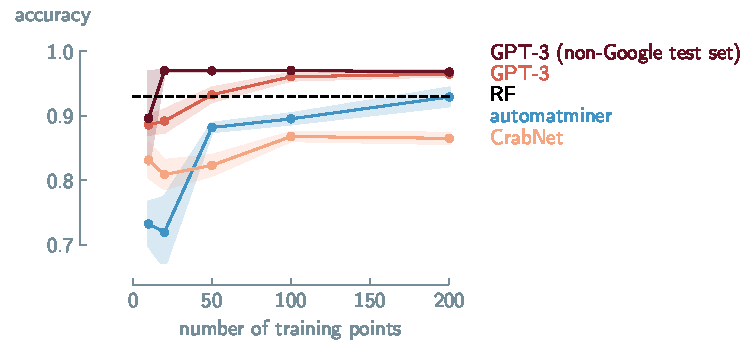
\includegraphics[width=1\textwidth]{figures/property_gptchem.pdf}
    \caption{\textbf{Fine-tuned \modelname{GPT-3} for predicting solid-solution formation in high-entropy alloys} Performance comparison of different \gls{ml} approaches as a function of the number of training points. Results are shown for \modelname{Automatminer} (blue), \modelname{CrabNet} transformer (orange),  fine-tuned \modelname{GPT-3} (red), with error bars showing standard error of the mean. The non-Google test set shows the fine-tuned \modelname{GPT-3} model tested on compounds without an exact Google search match (dark red). The dashed line shows performance using random forest. \modelname{GPT-3} achieves comparable accuracy to traditional approaches with significantly fewer training examples. Data adapted from \textcite{jablonka2024leveraging}}
    \label{fig:gptchem}
\end{figure}

\paragraph{\gls{lift}} \textcite{dinh2022lift} showed that reformulating regression and classification as \gls{qa} tasks enables the use of unmodified model architecture while improving performance (see \Cref{sec:fine-tuning} for a deeper discussion of \gls{lift}). 
In recognizing the scarcity of experimental data and acknowledging the persistence of this limitation, \textcite{jablonka2024leveraging} designed a \gls{lift}-based framework using \modelname{GPT-3} fine-tuned on task-specific small datasets (see \Cref{tab:property_prediction_models}). 
They seminally demonstrated that fine-tuned \modelname{GPT-3} can match or surpass specialized \gls{ml} models in various chemistry tasks. A key finding was fine-tuned \modelname{GPT-3}'s ability to generalize beyond training data. 
When tested on compounds absent from Google Search (and likely its training data), it performed well, proving that it was not simply recalling memorized information (see \Cref{fig:gptchem}).

In a follow-up to \textcite{jablonka2024leveraging}'s work, \textcite{vanherck2025assessment} systematically evaluated this approach across 22 diverse real-world chemistry case studies using three open-source models. They demonstrate that fine-tuned \glspl{llm} can effectively predict various material properties. For example, they achieved $96\%$ accuracy in predicting the adhesive free-energy of polymers, outperforming traditional \gls{ml} methods like random forest ($90\%$ accuracy). When predicting properties of monomers using \gls{smiles} notation, the fine-tuned models reached average accuracies of $84\%$ across four different properties. Particularly notable was the ability of \glspl{llm} to work with non-standard inputs, like in a protein phase separation study they did, where raw protein sequences could be directly input without pre-processing and achieve $95\%$ prediction accuracy. At the same time, when training datasets were very small (15 data points), the predictive accuracy of all fine-tuned models was lower than the random baseline (e.g. MOF synthesis). These case studies preliminarily demonstrate that these models can achieve predictive performance with some small datasets, work with various chemical representations (\gls{smiles}, \gls{mof}id, and \gls{iupac} names), and can outperform traditional \gls{ml} approaches for some material property prediction tasks.

In the materials domain, \modelname{LLMprop} fine-tunes \modelname{T5}\autocite{raffel2020exploring} to predict crystalline material properties from text descriptions generated by \modelname{Robocrystallographer}\autocite{ganose2019robocrystallographer}. By discarding \modelname{T5}’s decoder and adding task-specific prediction heads, the approach reduces computational overhead while leveraging the model’s ability to process structured crystal descriptions. The method demonstrates that natural language representations can effectively capture key material features, offering an alternative to traditional graph-based models like \glspl{gnn}.

Fine-tuning has been used to adapt \glspl{ssm} like Mamba (see \Cref{sec:example_architectures}). By pre-training on 91 million molecules, the Mamba-based model \modelname{$\text{O}_{SMI}-{\text{SSM}-}336\textit{M}$} outperformed transformer methods (\modelname{Yield-BERT}\autocite{krzyzanowski2025exploring}) in reaction yield prediction (e.g., Buchwald-Hartwig cross-coupling) and achieved competitive results in molecular property prediction benchmarks.\autocite{soares2025mamba-based} 

\paragraph{Foundational \glspl{gnn} and \glspl{mlip}} The fine-tuning approach has been applied to \enquote{foundational \glspl{gnn}} \autocite{sypetkowski2024scalability, shoghi2023molecules} and \glspl{mlip}, approaches distinct from \glspl{gpm}. For example, \textcite{shoghi2023molecules, sypetkowski2024scalability} show \gls{sota} performance on property prediction tasks.
\enquote{Foundational} \glspl{mlip} pre-trained on large datasets encompassing many chemical elements can be fine-tuned for specific downstream tasks \autocite{batatia2022mace}, such as calculating sublimation enthalpies of molecular crystal polymorphs \autocite{kaur2025data}.

\paragraph{Limitations} One central challenge is finding balance in datasets. In practical applications, researchers often have many more examples of poor-performing materials than optimal ones, resulting in unbalanced datasets that can diminish model performance. \textcite{vanherck2025assessment} point out that in the catalyzed cleavage reaction study, only $3.8\%$ of catalysts were labeled as \enquote{good}, forcing researchers to reduce their training set significantly to maintain balance. They also note that \glspl{llm} struggle with highly complex or noisy datasets, as seen in their study of catalytic isomerization, where even after hyperparameter optimization, the models failed to achieve meaningful predictive power due to the high noise in the experimental data and limited sample size. Finally, they note that although \glspl{llm} can work with different chemical representations, the choice of representation significantly impacts performance. For example, when predicting polymerization rates, models using \gls{smiles} notation significantly outperformed those using \gls{iupac} names, indicating that representation selection remains an important consideration.

Fine-tuning effectively adapts \glspl{llm} to specialized chemistry tasks, but its dependence on static datasets hinders adaptability to new or evolving knowledge. \gls{rag}, whose fundamentals are described in detail in \Cref{sec:rag}, overcomes these limitations by dynamically integrating external data sources, enabling more flexible and up-to-date reasoning.

\subsubsection{Agents}

Caldas Ramos et al.\ introduce \modelname{MAPI-LLM}, a framework that processes natural-language queries about material properties using an \gls{llm} to decide which of the available tools such as the Materials Project \gls{api}, the Reaction-Network package, or Google Search to use to generate a response. \autocite{Jablonka2023} \modelname{MAPI-LLM} employs a \gls{react} prompt (see \Cref{sec:arch_agents} to read more about \gls{react}), to convert prompts such as  \textit{\enquote{Is $Fe_2O_3$ magnetic?}} or \textit{\enquote{What is the band gap of Mg(Fe3O3)2?}} into queries for Materials Project \gls{api}. 
The system processes multi-step prompts through logical reasoning, for example, when asked \textit{\enquote{If Mn2FeO3 is not metallic, what is its band gap?}}, the \gls{llm} system creates a two-step workflow to first verify metallicity before retrieving the band gap.

Building on this foundation of agent-based materials querying, \textcite{chiang2024llamp} advanced the approach with \modelname{LLaMP}, a framework that employs \enquote{hierarchical} \gls{react} agents to interact with computational and experimental data. This \enquote{hierarchical} framework employs a supervisor-assistant agent architecture where a complex problem is broken down and tasks are delegated to domain-specific agents.  \modelname{LLaMP} addresses the challenge of hallucinations more effectively than standard \gls{llm} approaches by grounding responses in retrieved materials databases, retrieving materials data (e.g., crystal structures, elastic tensors) while counteracting systematic \gls{llm} biases in property predictions. These biases include the tendency for \glspl{llm} to overestimate certain properties like bulk moduli and to exhibit errors in bandgap predictions based on compositional patterns learned during training rather than physical principles.


\subsubsection{Core Limitations}\label{sec:property_core_limits}

\begin{figure}[htb]
    \centering
    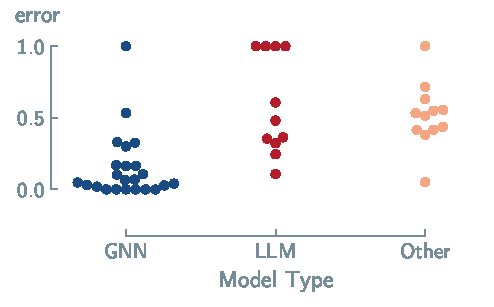
\includegraphics{figures/property_mattext.pdf}
    \caption{\textbf{Normalized error distributions for materials property prediction models across different architectures}. Each point represents the normalized error of a model on a specific property prediction task. Normalization was achieved with min/max values of each dataset to produce a range of errors between 0 and 1. The first column (blue) shows \gls{gnn} based models, the second column (red) displays \gls{llm} approaches, and the third column (orange) represents other baseline methods and \gls{sota} models including \modelname{CrabNet}. \autocite{Wang_2021} Lower values indicate better predictive performance. Data adapted from \textcite{alampara2024mattext}}
    \label{fig:property_limitations}
\end{figure}

\noindent \textcite{alampara2024mattext} introduced \modelname{MatText}, a framework for evaluating \glspl{lm} ability to predict properties of materials using text-based representations. 
Their findings indicate that current \glspl{llm} (including pre-trained \modelname{BERT} and fine-tuned \modelname{LLaMA-3-8B}) are effective for tasks relying purely on compositional information (e.g., element types and local bonding patterns), but struggle to leverage geometric or positional information encoded in text, as reflected in \Cref{fig:property_limitations}. 
This observation suggests that transformer-based architectures may be fundamentally limited to applications where spatial understanding is not required. 
Their experiments with data scaling and text representations reveal that increasing pre-training data or adding geometric details fails to improve downstream property prediction, challenging the conventional assumption that larger models and datasets universally enhance performance. \autocite{frey2023neural} 
Notably, \textcite{frey2023neural} demonstrated power-law scaling in chemical \glspl{llm}, but \modelname{MatText}'s results imply that such scaling may not overcome architectural biases against geometric reasoning in materials tasks.\autocite{gruver2024promises}

\subsection{Molecular and Material Generation} \label{sec:mol_generation}

\begin{figure}[htbp!]
    \centering
    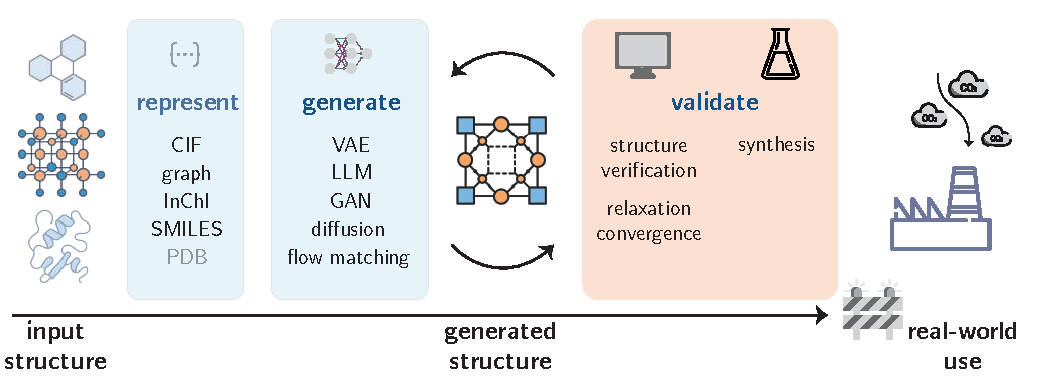
\includegraphics[width=1\textwidth]{figures/rescaled_figures/chemrev_figure21.pdf}
    \caption{\textbf{Pipeline for molecular and materials generation} The workflow begins with input structures represented in various formats, which are used to train \gls{ml} models to generate novel molecular and material structures. The generated structures should undergo a feedback loop through validation processes before being applied in the real world. Blue boxes indicate well-established areas of the pipeline with mature methodologies, while the red box represents critical bottlenecks.}
    \label{fig:generation}
\end{figure}

\noindent Early work in molecular and materials generation relied heavily on unconditional generation, where models produce novel structures without explicit guidance, relying solely on patterns learned from training data. For example, latent space sampling in autoencoders, where random vectors are decoded into new structures.\autocite{yoshikai2024novel} These methods excel at exploring chemical space broadly but lack fine-grained control. 
This limitation underscores the need for conditional generation, using explicit prompts or constraints (e.g., property targets, structural fragments), to steer \glspl{gpm} toward meaningful molecule or material designs. 
Beyond the generation step, as \Cref{fig:generation} shows, critical bottlenecks persist in synthesizability and physical consistency at the validation stage.

\subsubsection{Generation}\label{sec:generation}

\paragraph{Prompting}
While zero-shot and few-shot prompting strategies demonstrate promising flexibility for molecule generation, benchmark studies \autocite{guo2023large} reveal significant limitations that restrict their practical utility. \textcite{guo2023large} exposed fundamental gaps in \glspl{llm}' molecular design capabilities through a systematic evaluation. \modelname{GPT-4} was reported to produce chemically valid \gls{smiles} $89\%$ of the time but achieving less than $20\%$ accuracy in matching the target specifications. 
This result is far below specialized models like \modelname{MolT5}\autocite{edwards2022translation}. 
They conclude that this performance gap stems from \glspl{llm}' inadequate understanding of \gls{smiles} syntax and structure-property relationships. 
Subsequent work by \textcite{bhattacharya2024large} explored whether systematic prompt engineering could overcome these limitations, demonstrating that these prompts could guide \modelname{Claude 3 Opus} to generate chemically valid molecules ($97\%$ syntactic validity) with controlled modifications, including fine-grained structural changes (median Tanimoto similarity $0.67$--$0.69$) and predictable electronic property shifts (\SIrange{0.14}{0.27}{eV} \gls{homo} energy changes). Hybrid approaches like \modelname{FrontierX} extend this method with knowledge-augmented prompting, where \glspl{llm} generate both molecule predictions and explanations that are used to fine-tune smaller \glspl{lm}, with all resulting embeddings ultimately combined via hierarchical attention mechanisms to produce the final \gls{smiles} representation\autocite{srinivas2024crossing}. 
It showed improved accuracy over pure prompting strategies but sacrificed the generalizability that makes \glspl{llm} attractive, as the model requires re-training for each new molecular domain. 

\paragraph{Fine-Tuning} To overcome the limitations of prompting, fine-tuning has been adopted in molecular and materials generation, much like its use in property prediction with \gls{lift}-based frameworks (see \Cref{sec:fine-tuning} for a deeper explanation of \gls{lift} and \Cref{sec:prediction_FT} for a discussion of \gls{lift} applied to property prediction tasks). \textcite{yu2024llasmol} demonstrated that systematic fine-tuning in various chemical tasks including molecule generation from captions can improve performance while remaining parameter-efficient, using only $0.58\%$ of trainable parameters via \gls{lora}.

The molecule-caption translation task (\modelname{Mol2Cap}), which involves generating textual descriptions from molecular representations and vice versa (Cap2Mol), has become a standard benchmark for evaluating \glspl{gpm} for molecule generation. \autocite{edwards2022translation} Under the \enquote{Mol2Cap}/\enquote{Cap2Mol} task paradigm, \gls{icma} avoids domain-specific pre-training by combining retrieval-augmented in-context learning with fine-tuning on \gls{icl} examples.\autocite{li2025large} 
On the ChEBI-20\autocite{edwards2021text2mol} and PubChem324k\autocite{liu2023molca} datasets, \gls{icma} nearly doubles baseline performance, with \gls{icma} powered by\modelname{Mistral-7B} achieving a 0.581 \gls{bleu} score in \modelname{Mol2Cap} and $46.0\%$ exact match in \modelname{Cap2Mol}.\autocite{li2025large} 
However, its reliance on retrieved examples raises concerns about generalization to novel scaffolds. 
Similarly, \modelname{MolReFlect} enhances fine-grained alignment through a teacher-student framework, where a larger \gls{llm} (e.g., \modelname{GPT-4}) extracts substructure-aware captions to guide a smaller model (\modelname{Mistral-7B}), improving \modelname{Cap2Mol} accuracy while reducing hallucinations.\autocite{li2024molreflect} 
Meanwhile, \modelname{PEIT-LLM} extends the task to property-conditioned generation, using instructions (\gls{smiles}-text-property tuples) to optimize for captioning and prediction jointly.\autocite{lin2025property} 

Fine-tuned \glspl{lm} have shown promise in molecule and materials generation. 
However, their reliance on decoding and \gls{smiles}/\gls{selfies} representations introduces fundamental limitations: degeneracy (multiple valid \gls{smiles} for the same molecule) and difficulty capturing complex structural relationships implicit in textual descriptions.

\paragraph{Diffusion and Flow Matching} Diffusion and flow-based models operate directly on latent representations, enabling more flexible generation of diverse and novel structures.\autocite{zhu20243m-diffusion} Moreover, emerging hybrid architectures combine the strengths of \glspl{llm} with diffusion and flow matching models to overcome the limitations of each paradigm individually \autocite{sriram2024flowllm}.

Beyond text-based representations, \modelname{llamole} introduced a multimodal \gls{llm} approach capable of text and graph generation by integrating a base \gls{llm} with graph diffusion transformers and graph neural networks for multi-conditional molecular generation and retrosynthetic planning. Specifically they used different trigger (\texttt{<design>} and \texttt{<retro>}) and query (\texttt{<query>}) tokens for switching between them and improved success in synthesis success rates from  $5\%$ to $35\%$ . \autocite{liu2024multimodal}

A unique challenge with crystalline materials is generating a material that possesses both discrete (atom type) and continuous (atomic position and lattice geometry) variables. \textcite{sriram2024flowllm} developed \modelname{FlowLLM} to address this challenge. They recognized that the respective strengths of \glspl{llm}, modeling discrete values and conditional prompting, and denoising models, modeling continuous values and equivariances, could be combined to create a hybrid architecture. 
A fine-tuned \gls{llm} is used to learn an effective base distribution of metastable crystals via text-based representations, which is then iteratively refined through \gls{rfm} to optimize atomic coordinates and lattice parameters.\autocite{sriram2024flowllm}

\paragraph{Reinforcement Learning and Preference Optimization}

Translating \gls{gpm} generated outputs to the real world requires designing molecules and materials with specific target properties. \gls{rl} and preference optimization techniques\autocite{lee2024fine-tuning} have emerged as powerful solutions for this challenge. For instance, \textcite{jang2025can} combined \gls{sft} and \gls{rl} using \gls{ppo} to generate diverse molecular sequences auto-regressively. 
This approach excels in exploring a broad chemical space, but incurs high computational costs due to its reliance on iterative, sequence-based generation. 
In contrast, \textcite{cavanagh2024smileyllama} employed \gls{dpo} with \gls{sft} to fine-tune \glspl{llm} for molecular design, leveraging \gls{smiles} representations to optimize drug-like properties (e.g., hydrogen bond donors/acceptors and LogP).
While \gls{dpo} reduces computational overhead in comparison to \gls{ppo}, it trades off molecular diversity, a key strength of the work by \textcite{jang2025can}, due to the inherent constraints of preference-based fine-tuning.

Beyond these methods, \gls{era} introduces a different optimization paradigm. \autocite{chennakesavalu2025aligning} Unlike \gls{ppo} or \gls{dpo}, \gls{era} uses gradient-based objectives to guide word-by-word generation with explicit reward functions, converging to a physics-inspired probability distribution that allows fine control over the generation process. 
In single-property optimization tasks, \gls{era} successfully aligned molecular transformers to generate compounds with targeted chemical properties (QED, LogP, ring count, molar refractivity) while maintaining $59-84\%$ chemical validity without regularization. For multi-objective optimization, it achieved precise control over property trade-offs using weighted energy functions.

\textcite{calanzone2025mol-moe} also address the challenge of multi-objective molecular generation with \modelname{MOL-MOE}, a \gls{moe} framework (see \Cref{sec:arch-moes} to learn more about \gls{moe} architectures). \modelname{MOL-MOE} dynamically combines property-specific expert models at test time using preference-guided routers toward drug-relevant molecular properties enabling flexible steering across multiple objectives without re-training. Compared to alternatives like \modelname{MORLHF}\autocite{zhou2024one-preference-fits-all}, \gls{sft} with rewards-in-context, and simple model merging such as Rewarded Soups\autocite{rame2023rewarded}), \modelname{MOL-MOE} achieves superior performance in both property optimization and steerability---particularly in out-of-distribution scenarios where other methods struggle. 

\modelname{CrystalFormer-RL} uses \gls{rl} fine-tuning to optimize \modelname{CrystalFormer}\autocite{cao2024space}, a transformer-based crystal generator, with rewards from discriminative models (e.g., property predictors)\autocite{cao2025crystalformer-rl}. \gls{rl} improves stability (lower energy above convex hull) and enables property-guided generation (e.g., high dielectric constant + band gap). Here, \gls{rl} fine-tuning is shown to outperform supervised fine-tuning, enhancing both novel material discovery and retrieval of high-performing candidates from the pre-training dataset.

\paragraph{Agents} Agent-based frameworks leveraging \glspl{llm}, deeply explained in \Cref{sec:agents}, have emerged as approaches for autonomous molecular and materials generation, demonstrating capabilities that extend beyond simple prompting or fine-tuning by incorporating iterative feedback loops, tool integration, and human-\gls{ai} collaboration. 
The \modelname{dZiner} framework implements this approach for the inverse design of materials, where agents input initial \gls{smiles} strings with optimization task descriptions and generate validated candidate molecules by retrieving domain knowledge from the literature.\autocite{ansari2024dziner} 
It also uses domain-expert surrogate models to evaluate the required property in the new molecule/material. 
These surrogate models are highly customizable to the desired property and give the user the option to train their own \gls{ml} model or using an existing \gls{sota} model. \textcite{ansari2024dziner} demonstrated \modelname{dZiner}'s capabilities in generating surfactants for critical micelle concentration reduction, WDR5 inhibitors, and optimizing \gls{mof} organic linkers for \ce{CO2} adsorption. The \modelname{CLADD} framework adopts a \gls{rag}-enhanced multi-agent approach where specialized teams including \enquote{Planning}, \enquote{Knowledge Graph}, and \enquote{Molecular Understanding} collaborate to dynamically retrieve and integrate external biochemical knowledge for drug discovery tasks without requiring domain-specific fine-tuning.\autocite{lee2025rag-enhanced}

\subsubsection{Validation}
\paragraph{General validation} The most fundamental validation approaches use cheminformatics tools like \modelname{RDKit} to verify molecular validity. \modelname{RDKit} provides robust tools for validating molecules through its ability to parse and sanitize molecules from \gls{smiles} strings. 
If a step in the \gls{smiles} to structure conversion process fails, then the molecule is considered invalid. More sophisticated validation involves quantum mechanical calculations to compute molecular properties such as formation energies\autocite{kingsbury2022flexible}. These computationally expensive operations provide deeper insights into whether generated structures are viable. Models are also evaluated for their ability to generate unique molecules by calculating the proportion of unique molecules in generated sets, often using molecular fingerprints or structural descriptors. 

The gold standard for validation is experimental synthesis, but significant gaps exist between computational generation and laboratory realization. Preliminarily, metrics like Tanimoto similarity and Fréchet ChemNet distance \autocite{preuer2018frechet} quantify structural resemblance, which can indicate synthetic feasibility when training data consists of known compounds. Retrosynthesis prediction algorithms attempt to bridge this gap by evaluating synthetic accessibility and proposing potential synthesis routes (see \Cref{sec:retrosynthesis}). 
However, these methods still face limitations in accurately predicting real-world synthesizability \autocite{zunger2019beware}.


\paragraph{Conditional Generation Validation} Beyond establishing the general validity of generated molecules, evaluation methods can assess both their novelty relative to training data and their ability to meet specific design goals. For inverse design tasks, such as optimizing binding affinity or solubility, the \textit{de novo} molecule generation benchmark GuacaMol differentiates between \textit{distribution-learning} (e.g., generating diverse, valid molecules) and \textit{goal-directed} optimization (e.g., rediscovering known drugs or meeting multi-objective constraints) \autocite{brown2019guacamol}. 
In the materials paradigm, frameworks such as \modelname{MatBench Discovery} evaluate analogous challenges such as stability, electronic properties, and synthesizability, but adapt metrics to periodic systems, such as energy above hull or band gap prediction accuracy\autocite{riebesell2025framework}. Recently, they introduced the \enquote{discovery acceleration factor}, which quantifies how effective a model is at finding stable structures relative to a random baseline.

\subsection{Retrosynthesis}\label{sec:retrosynthesis}

The practical utility of \glspl{gpm} for generating molecules and materials remains limited by a persistent gap in their synthetic feasibility. Early work by \textcite{schwaller2021mapping} laid important groundwork by demonstrating how attention-based neural networks can learn meaningful representations of chemical reactions, enabling accurate classification and prediction of reaction outcomes. Their model, trained on millions of reactions from patent and literature data, showed that learned reaction embeddings were capable of capturing nuanced chemical relationships. 

Recent efforts have built on this foundation by integrating synthesizability directly into molecular and materials generation pipelines that leverage both domain-specific tools and \glspl{gpm}. For example, \textcite{sun2025synllama} adapted \modelname{Llama-3.1-8B} and \modelname{Llama-3.2-1B} to predict retrosynthetic pathways and identify commercially available building blocks for experimentally validated SARS-CoV-2 Mpro inhibitors. 
Similarly, \textcite{liu2024multimodal} introduced a multimodal framework that combines reaction databases with chemical intuition encoded in \glspl{llm}, improving the prioritization of high-yield, low-cost synthetic routes.

More recent work has explored how fully fine-tuned \glspl{llm} can serve as comprehensive chemistry assistants for experimental guidance. \textcite{zhang2025large} developed \modelname{Chemma}, a fine-tuned \modelname{LLaMA-2-7B} model trained on 1.28 million chemical reaction question-answer pairs. Through an active learning framework that incorporates experimental feedback (see \Cref{sec:rl} to learn more about \gls{rl}), human-\modelname{Chemma} collaboration successfully optimized an unreported Suzuki-Miyaura cross-coupling reaction within only 15 experimental runs.

Predictive retrosynthesis has also extended to the inorganic domain. \textcite{kim2024large} demonstrated that fine-tuned \modelname{GPT-3.5} and \modelname{GPT-4} can predict both the synthesizability of inorganic compounds from their chemical formulas and select appropriate precursors for synthesis, achieving performance comparable to specialized \gls{ml} models with minimal development time and cost. 
In a follow-up work, they extended this approach to structure-based predictions of inorganic crystal polymorphs, where \glspl{llm} provided human-readable explanations for their synthesizability assessments\autocite{kim2025explainable}. 
Notably, their structure-aware models correctly identified twelve hypothetical compounds as non-synthesizable despite their thermodynamic stability, perfectly matching experimental outcomes where synthesis attempts failed.

Beyond retrosynthetic prediction, \glspl{llm} have also been deployed as reasoning engines for autonomous design. \textcite{bran2024augmenting} developed \modelname{ChemCrow}, an \gls{llm}-based system that autonomously plans and executes the synthesis of novel compounds by integrating specialized tools like a retrosynthesis planner (see \Cref{sec:planning} to read more about this capability of \modelname{ChemCrow} and its limitations) and reaction predictors. This approach mirrors the iterative experimental design cycle employed by human chemists, but is equipped with the scalability of automation. Notably, systems like \modelname{ChemCrow} rely on high-quality reaction data to ground their reasoning in empirically viable chemistry, which, depending on the design space, could be a limitation.

\subsection{LLMs as Optimizers} \label{sec:llm-optimizers}

\begin{figure}[htb]
    \centering
    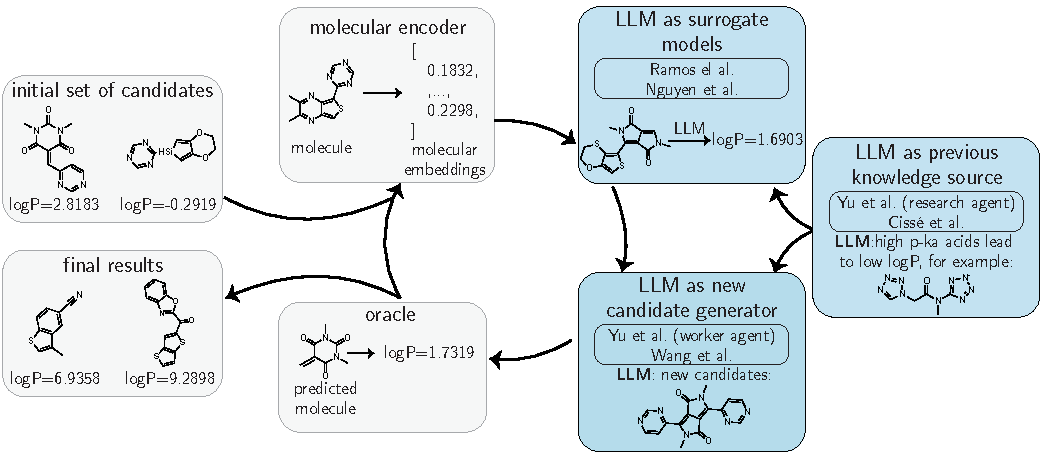
\includegraphics[width=1\textwidth]{figures/rescaled_figures/chemrev_figure22.pdf}
    \caption{\textbf{Overview of the iterative optimization loop that mirrors the structure of the optimization section}. The blue boxes contain the different roles that the \glspl{llm} play in the loop, and which are described in the main text. References in which the use of \glspl{llm} for that step are detailed inside the small boxes inside each of the components of the loop. The example shown is about obtaining molecules with high \texttt{logP}.}
    \label{fig:optimization}
\end{figure}

Discovering novel compounds and reactions in chemistry and materials science has long relied on iterative trial-and-error processes rooted in existing domain knowledge \autocite{Taylor2023brief}. While, as explained in \Cref{sec:retrosynthesis}, those methods are used to accelerate this process, optimization methods help improve conditions, binding affinity, etc.
But these approaches are slow and labor-intensive. 
Traditional data-driven methods aimed to address these limitations by combining predictive \gls{ml} models with optimization frameworks such as \gls{bo} or \glspl{ea}. 
These frameworks balance exploration of uncharted regions in chemical space with exploitation of known high-performing regions \autocite{Li2024sequential, Hse2021gryffin, Shields2021bayesian, Griffiths2020constrained, RajabiKochi2025adaptive}.

Recent advances in \glspl{llm} have unlocked potential for addressing optimization challenges in chemistry and related domains \autocite{fernando2023promptbreeder0, yang2023large, chen2024instruct}. 
A key strength of \glspl{llm} lies in their capacity to frame optimization tasks through natural language, which enhances knowledge incorporation, improves candidate comparisons, and increases interpretability. 
This aligns well with chemical problem-solving, where complex phenomena, such as reaction pathways or material behaviors, are often poorly captured by standard nomenclature; however, they can still be intuitively explained through natural language. 
Moreover, \glspl{gpm}' general capabilities provide flexibility beyond classical methods, which have to be trained from scratch if the optimization problem or any of its variables changes.
By encoding domain-specific knowledge---including reaction rules, thermodynamic principles, and structure-property relationships---into structured prompts, \glspl{llm} can synergize expertise with their ability to navigate complex chemical optimization problems.

Current \gls{llm} applications in chemistry optimization vary in scope and methodology. 
Many studies integrate \glspl{llm} into \gls{bo} frameworks, where models guide experimental design by predicting promising candidates \autocite{rankovic2023bochemian}. Others employ \glspl{ga} or hybrid strategies that combine \gls{llm}-generated hypotheses with computational screening \autocite{cisse2025language0based}.  

\subsubsection{LLMs as Surrogate Models}

A prominent \gls{llm}-driven strategy positions these models as surrogate models within optimization loops. Typically implemented as \gls{gpr}, surrogate models learn from prior data to approximate costly feature-outcome landscapes, which are often computationally and time-consuming to evaluate, thereby guiding the acquisition.
\glspl{llm} offer major advantages in this role primarily through strong low-data performance. 
Their \gls{icl} capability enables task demonstration with minimal prompt examples while leveraging chemical knowledge from pre-training to generate accurate predictions. 
This allows \glspl{gpm} to compensate for sparse experimental data effectively.

\textcite{ramos2023bayesian} demonstrated the viability of this paradigm through a simple yet effective framework that combines \gls{icl} using only one example in the prompt with a \gls{bo} workflow. 
Their \gls{bo}-\gls{icl} approach uses few-shot examples formatted as question-answer pairs, where the \gls{llm} generates candidate solutions conditioned on prior successful iterations. 
These candidates are ranked using an acquisition function, with top-$k$ selections integrated into subsequent prompts to refine predictions iteratively. 
Remarkably, this method achieved high performance in optimizing catalytic reaction conditions, even matching the top-1 accuracies observed in experimental benchmarks. This emphasizes the potential of \glspl{llm} as accessible, \gls{icl} optimizers when coupled with well-designed prompts.

To address limitations in base \glspl{llm}’ inherent chemical knowledge---particularly their grasp of specialized representations like \gls{smiles} or structure-property mappings---\textcite{yu2025collaborative} introduced a hybrid architecture augmenting pre-trained \glspl{llm} with task-specific embedding and prediction layers. 
These layers, fine-tuned on domain data, align latent representations of input-output pairs (denoted as \texttt{<x>} and \texttt{<y>} in prompts), enabling the model to map chemical structures and properties into a unified, interpretable space. Crucially, the added layers enhance chemical reasoning without sacrificing the flexibility of \gls{icl}, allowing the system to adapt to trends across iterations, similarly to what was done by \textcite{ramos2023bayesian}. 
In their evaluations of molecular optimization benchmarks, such as the \gls{pmo} \autocite{gao2022sample}, they revealed improvements over conventional methods, including \gls{bo}-\gls{gp}, \gls{rl} methods, and \gls{ga}.

\textcite{yu2025collaborative} further highlighted the framework’s extensibility to diverse black-box optimization challenges beyond chemistry. 
This represents one of the most important advantages of using \glspl{llm} as orchestrators of the optimization process. 
The flexibility of natural language in this process enables the procedure to be applied to any optimization process. 
In contrast, classical methods are constrained to the specific task for which they are designed due to the need to train the surrogate model.

\subsubsection{LLMs as Next Candidate Generators}

Recent studies demonstrate the potential of \glspl{llm} to enhance \glspl{ea} \autocite{lu2024generative} and \gls{bo} \autocite{amin2025towards} frameworks by leveraging their embedded chemical knowledge and ability to integrate prior information, thereby reducing computational effort while improving output quality.
Within \glspl{ea}, \glspl{llm} refine molecular candidates through mutations (modifying molecular substructures) or crossovers (combining parent molecules). 
In \gls{bo} frameworks, they serve as acquisition functions, utilizing surrogate model predictions---both mean and uncertainty---to select optimal molecules or reaction conditions for evaluation.

For molecule optimization, \textcite{yu2025collaborative} introduced \modelname{MultiModel}, a dual-\gls{llm} system where one model proposes candidates and the other supplies domain knowledge (see \Cref{sec:opt-llm-know-source}). 
By fine-tuning the \enquote{worker} \gls{llm} to recognize molecular scaffolds and target properties, and expanding the training pool to include a million-size pre-training dataset, they achieved hit rates exceeding $90\%$. 
Similarly, \textcite{wang2024efficient} developed \modelname{MoLLEO}, integrating an \gls{llm} into an \gls{ea} to replace random mutations with \gls{llm}-guided modifications. Here, \modelname{GPT-4} generated optimized offspring from parent molecules, significantly accelerating convergence to high fitness scores. 
Notably, while domain-specialized models (\modelname{BioT5}, \modelname{MoleculeSTM}) underperformed, the general-purpose \modelname{GPT-4} excelled---a finding that underscores the context-dependent utility of \glspl{llm}

In a related approach, \textcite{lu2024generative} showed that well-designed prompts---incorporating task-specific constraints, objectives, and few-shot examples---enable general \glspl{llm} (\modelname{Claude\--3.5-Sonnet}, \modelname{o1-preview}) to generate high-quality candidates without fine-tuning, outperforming both random selection and vanilla \glspl{ga} in functional \gls{tmc} design.

\subsubsection{LLMs as Prior Knowledge Sources} \label{sec:opt-llm-know-source}

A key advantage of integrating \glspl{llm} into optimization frameworks is their ability to encode and deploy prior knowledge within the optimization loop. 
As illustrated in \Cref{fig:optimization}, this knowledge can be directed into either the surrogate model or candidate generation module, significantly reducing the number of optimization steps required through high-quality guidance.

For example, \textcite{yu2025collaborative} deployed a \enquote{research} agent that leverages \modelname{Google} search and \modelname{RDKit} to verify and rank molecules generated by \enquote{worker} agents against target features and properties. 
Their results demonstrate substantial improvements when this filtering mechanism is applied.

Similarly, \textcite{cisse2025language0based} introduced \modelname{BORA}, which contextualizes conventional black-box \gls{bo} using an \gls{llm}. \modelname{BORA} maintains standard \gls{bo} as the core driver but strategically activates the \gls{llm} when progress stalls. 
This leverages the model’s \gls{icl} capabilities to hypothesize promising search regions and propose new samples, regulated by a lightweight heuristic policy that manages costs and incorporates domain knowledge (or user input). 
Evaluations on synthetic benchmarks such as the catalyst optimization task for hydrogen generation show that \modelname{BORA} accelerates exploration, improves convergence, and outperforms existing \gls{llm}-\gls{bo} hybrids.

To enhance the task-specific knowledge of the \gls{llm} generating feedback, \textcite{zhang2025large} fine-tuned a \modelname{Llama-2-7B} model using a multitask \gls{qa} dataset. This dataset was created with instructions from \modelname{GPT-4}. 
The resulting model served as a human assistant or operated within an active learning loop, thereby accelerating the exploration of new reaction spaces (see \Cref{sec:retrosynthesis}). 
However, as the authors note, even this task-specialized \glspl{llm} produces suboptimal suggestions for optimization tasks. 
They remain prone to hallucination and cannot assist with unreported reactions, but still, they improve for most of the applications, using pure classical methods.

\subsubsection{How to Face Optimization Problems?}

Published works explore different ways of using \glspl{llm} for optimization problems in chemistry, from simple approaches, such as just prompting the model with some initial random set of experimental candidates and iterating \autocite{ramos2023bayesian}, to fine-tuning models in \gls{bo} fashion \autocite{rankovic2025gollum0}. 
The most efficient initial point is by relying entirely on a \gls{icl} approach, which allows one to obtain a first signal rapidly. 
Such initial results will enable to determine whether a more complex, computationally intensive approach is necessary or whether prompt engineering is reliable enough for the application. 
Fine-tuning can be used as a way to enhance the chemical knowledge of the \glspl{llm} and can lead to improvements in optimization tasks where the model requires such knowledge to choose or generate better candidates. 
Fine-tuning might not be a game-changer for other approaches that rely more on sampling methods \autocite{wang2025llm0augmented}.

While some initial works showed that \glspl{llm} trained specifically on chemistry perform better for optimization tasks \autocite{kristiadi2024sober}, other works showed that a \gls{gpm} such as \modelname{GPT-4} combined with an \gls{ea} outperformed all other models \autocite{wang2024efficient}.
Is it better to incorporate a general model or a chemistry \gls{lm} into the optimization frameworks?
We hypothesize that for models of the same size (in number of parameters) and similar training size---attending to \glspl{pflop}---a chemical \gls{lm} (a specialized model) will consistently outperform general models. 
If the models differ significantly in size, the larger model will typically perform better.

